\documentclass[12pt,a4paper]{article}

%\usepackage[left=2cm, right=2cm, top=4cm, bottom=2cm]{geometry}
\usepackage[utf8]{inputenc}
\usepackage[spanish]{babel}
\usepackage{enumitem}
\usepackage{amsmath}
\usepackage{tikz}

\usepackage{hyperref}
\hypersetup{
    colorlinks=true,
    linkcolor=blue,
    filecolor=magenta,
    urlcolor=cyan,
}

\begin{document}

\begin{titlepage}
	\centering
	{\scshape\LARGE Universidad Nacional Autónoma de México \par}
	\vspace{1cm}
	{\scshape\Large Computación Distribuida\par}
	\vspace{1cm}
	{\huge\bfseries Algoritmos Autorregulables\par}
	\vspace{1cm}
    {\Large\itshape Jerónimo Almeida Rodríguez \par}
    \vspace{.5cm}
	{\Large\itshape Edgar Quiroz Castañeda \par}
    \vspace{.5cm}
	{\Large\itshape Naomi Reyes ...\par}
	\vfill
	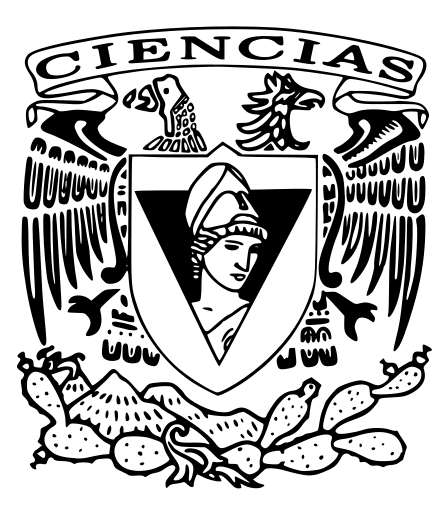
\includegraphics[width=0.5\textwidth]{escudo_f-ciencias.png}
	\vfill

	{\large Viernes 14 de Diciembre del 2018 \par}
\end{titlepage}

	\pagebreak
	\setlength{\voffset}{-0.75in}
	\setlength{\headsep}{5pt}


\begin{center}
		\textsc{\huge Algoritmos Autorregulables\\}
		\textit{Jerónimo Almeida, Edgar Quiroz, Naomi Reyes\\}
        14/12/2018
\end{center}




\section{Introducción}{
    Los algoritmos autorregulables son aquellos tienen la propiedad de que todos los procesos que ejecuten dicho algoritmo tiendan eventualmente a alcanzar un estado válido sin importar el estado actual en el que se encuentren, es decir, que pueden iniciar en cualquier estado arbitrario no válido o en caso de que haya ocurrido algún error que altere el estado, que el proceso llegue a un estado válido. Este estado válido se define en términos de los requerimientos del sistema.
\subsection{Motivación}{
    Con un algoritmo autorregulable buscamos que el sistema se recupere de un error sin intervención humana, es decir que dado un estado global arbitrario (particularmente uno que sea erróneo), dar un algoritmo que haga que el estado global eventualmente se vuelva válido.\\
    \indent Saludos
}
\subsection{Especificación}{
    De los algoritmos autorregulables, sabemos que en general, un proceso no puede determinar "desde adentro" si el estado en el que está es válido o no, por lo que tener una bandera o indicador de la validez del estado no es la mejor opción, ya que algún agente malicioso podría cambiar esta bandera y hacer que el proceso crea que ha alcanzado un estado válido aunque esto no sea cierto. Esta es la razón por la que estos algoritmos no terminan, pues de hacerlo podrían terminar en un estado que no sea válido. En cambio, lo que hacen es que convergen hacia un estado válido, es decir que el proceso, por medio de esta subrutina, modifica su estado de tal manera que con cada ejecución se acerque mas a lo que es el estado válido. De esto, tenemos la garantía de que eventualmente el estado global del sistema va a ser válido. De igual manera, sabemos que una vez alcanzado un estado válido, mientras no hayan errores, este estado válido se mantendrá por el resto de la ejecución. Una ventaja de que el proceso no termine, es que si algun proceso comete un error, puede recuperarse de ese error y regresar a un estado válido.

}
\subsection{Modelo}{}
}
\section{Pase de Token en un Anillo}{}
\section{Sincronizadores}{
\subsection{Generalidades de sincronizadores}{}

\subsection{Sincronizador $\alpha$}{}

\subsection{Sincronizador autorregulable}{}

    \subsubsection{Regla Simple}{}

    \subsubsection{Segunda Regla}{}

    \subsubsection{Regla Óptima}{}
}
\section{Conclusión}{}

\begin{thebibliography}{}

\bibitem[Asp18]{Asp18}
James Aspnes. Notes on Theory of Distributed Systems.
\href{http://www.cs.yale.edu/homes/aspnes/classes/465/notes.pdf}
{http://www.cs.yale.edu/homes/aspnes/classes/465/notes.pdf}, October 2018.

\end{thebibliography}
\end{document}
